\documentclass[12pt,english]{article}
\usepackage{geometry}[margin=2]
\usepackage{blindtext}
\usepackage{enumerate}
\usepackage{parskip} 
\usepackage{siunitx}
\usepackage{amsmath}
\usepackage{amsfonts}
\usepackage{amssymb}
\usepackage{hyperref}
\usepackage{listings}
\usepackage{inconsolata}
\usepackage{parskip}
\usepackage{graphicx}
\usepackage{wrapfig}
\graphicspath{./images}
\author{
    Cole Johnson: \texttt{cole.johnson.@student.nmt.edu}
    \\ 
    John Runyon: \texttt{john.runyon@student.nmt.edu}
}
\title{
    CSE441: Project Proposal\\
    \large{Cryptanalysis of Hash Functions}
}
\begin{document}
\maketitle
\section*{Introduction and Outline of Project}
\subsection{The Basics of Hash Functions}
Hashing, as an overall process, is a function that maps
plaintext data of any length into a fixed-length ciphertext
output--often called a digest. Hash functions, unlike encryption,
destroy information encoded in the plaintext, which means
the function is one-way and cannot be reversed to obtain
the plaintext again.

\begin{wrapfigure}{r}{0.5\textwidth}
    \begin{center}
      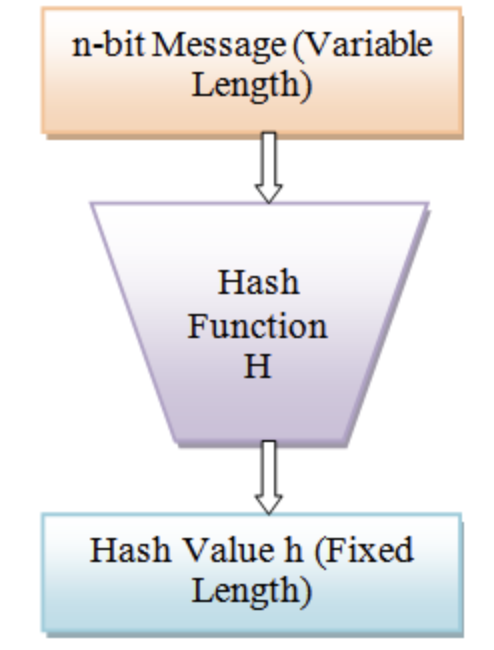
\includegraphics[clip=true,height=5cm, width=0.3\textwidth]{images/hash_function.png}
    \end{center}
    \caption{Basic diagram of a hash function}
  \end{wrapfigure}

Hash functions are a widely used cryptographic algorithm.
They can be used for a variety of purposes, such as
data integrity verification, password storage, and digital
fingerprint/signatures, and data indexing (often called hash-tables).
Since hash functions serve vital purposes in modern cryptography
and computer science, knowing the important mathematical properties
of a hash function (and how these can be implemented in programs)
is critical to understanding their function. Once the function and
real-world implementation

\subsection{Outline of Project}
Here is the sections of the project, along with a small description 
of what each of the sections would cover:
\begin{enumerate}[{\bf (a.)}]
    \item Introduction to Hash Functions
    \begin{enumerate}
        \item Basics of Hash Functions
        \item Modern and Classic Applications of Hash Functions
        \item Hash Functions Examples (MD5, SHA-256, Tornado)
    \end{enumerate} 
    \item Properties of Hash Functions
    \begin{enumerate}
        \item One-way Function (Pre-Image Resistance)
        \item Target Collision Resistance (2nd Pre-Image Resistance)
        \item Deterministic
        \item Avalanche Effect
        \item Computational Speed
    \end{enumerate}
    \item Cryptanalysis and Attacks on Cryptographic Hash Functions
    \begin{enumerate}
        \item Brute-Force Attacks
        \item One-way Function Inversion
        \item 2nd Pre-Image Resistance Attack
        \item Collision Attack
    \end{enumerate}
\end{enumerate}
\end{document}
